\chapter{Control hormonal de la reproducción}\label{ch:b2:reproductive-hormones}

Cada mes, con un calendario que se mantiene con un margen de uno o dos
días durante treinta años, madura un \omterm{def:b2:mammal-reproduction:ovary}{folículo}, se libera un óvulo, el
revestimiento del útero se construye y después, salvo que haya llegado un
embrión, se desprende. Ningún reloj del cuerpo late a ese ritmo; el ritmo
surge de una conversación entre tres órganos --- el hipotálamo, la
hipófisis y el ovario --- en la que cada hormona controla la liberación de
la siguiente y la última controla la primera. Este capítulo desmonta esa
conversación: el eje que gobierna ambos sexos, el control tónico del
\omterm{def:b2:mammal-reproduction:testis}{testículo}, el control cíclico del ovario con su notable paso de la
retroalimentación negativa a la positiva, y las maneras en que el eje es
anulado por el embarazo, por los fármacos y por la clínica.

\section{El eje}

\begin{definition}[El eje hipotálamo-hipófisis-gónadas]\label{def:b2:reproductive-hormones:axis}
\index{hormona liberadora de gonadotropinas}\index{hormona luteinizante}\index{hormona foliculoestimulante}\index{retroalimentación negativa!hormonal}
Las neuronas del \emph{hipotálamo} secretan \emph{GnRH} (hormona
liberadora de gonadotropinas, un péptido de diez aminoácidos) hacia los
pequeños vasos porta que llegan a la \emph{adenohipófisis}, en breves
\emph{pulsos} cada una o dos horas. La GnRH hace que la hipófisis secrete
a la circulación general dos hormonas glucoproteicas, las
\emph{gonadotropinas} \emph{LH} (hormona luteinizante) y \emph{FSH}
(hormona foliculoestimulante). Estas actúan sobre las \emph{gónadas}: la
LH sobre las células que fabrican esteroides (\omterm{def:b2:mammal-reproduction:testis}{células de Leydig}, de la
teca y lúteas), la FSH sobre las células que nutren a los gametos
(\omterm{def:b2:mammal-reproduction:testis}{células de Sertoli} y de la granulosa). Las gónadas responden con
esteroides --- \emph{testosterona}, \emph{estradiol},
\emph{progesterona} --- y con el péptido \emph{inhibina}, que ejercen una
retroalimentación sobre el hipotálamo y la hipófisis: los esteroides
sobre ambos, sobre todo \emph{negativa}; la inhibina solo sobre la FSH.
El resultado es un bucle regulado en el que la producción de la gónada
se mantiene en un valor de consigna, y el mismo diseño de tres niveles
gobierna el tiroides y la corteza suprarrenal. Los mecanismos por los que
estas hormonas actúan sobre sus células son el tema del
\cref{ch:b2:cell-signalling}.
\end{definition}

\begin{omfigure}
\begin{tikzpicture}[every node/.style={font=\scriptsize}, >=stealth]
  \node[draw, rounded corners, fill=omDef!15, align=center, minimum width=3cm] (hyp) at (0,4.2) {hipotálamo\\GnRH, en pulsos};
  \node[draw, rounded corners, fill=omDef!15, align=center, minimum width=3cm] (pit) at (0,2.2) {adenohipófisis\\LH y FSH};
  \node[draw, rounded corners, fill=omProp!20, align=center, minimum width=3cm] (gon) at (0,0) {gónada\\esteroides, inhibina};
  \node[draw, rounded corners, fill=omExo!25, align=center, minimum width=3cm] (tar) at (5.2,0) {tejidos diana\\gametogénesis, conductos,\\caracteres secundarios};
  \draw[->, thick] (hyp) -- (pit) node[midway, right] {vasos porta};
  \draw[->, thick] (pit) -- (gon) node[midway, right] {sangre};
  \draw[->, thick] (gon) -- (tar);
  \draw[->, thick, omThm] (gon.west) .. controls (-3.0,0) and (-3.0,2.2) .. (pit.west);
  \draw[->, thick, omThm] (gon.west) .. controls (-4.6,0) and (-4.6,4.2) .. (hyp.west);
  \node[omThm, anchor=east, align=right] at (-3.9,1.2) {hacia la hipófisis:\\esteroides $(-)$,\\inhibina $(-)$ sobre la FSH};
  \node[omThm, anchor=east, align=right] at (-3.9,3.6) {hacia el hipotálamo:\\esteroides $(-)$\\(estradiol $(+)$\\a mitad del ciclo)};
\end{tikzpicture}

{\small El eje: la GnRH hipotalámica estimula la LH y la FSH hipofisarias,
que estimulan la gónada; los esteroides y la inhibina de la gónada ejercen
una retroalimentación negativa sobre los dos niveles superiores ---
salvo la breve retroalimentación positiva del estradiol que desencadena
la \omterm{def:b2:mammal-reproduction:ovary}{ovulación}.}
\end{omfigure}

\begin{proposition}[Por qué importan los pulsos]\label{prop:b2:reproductive-hormones:pulses}
\index{secreción pulsátil}\index{desensibilización de receptores}
La hipófisis solo responde a la GnRH si esta llega en pulsos. Una célula
expuesta de forma continua a una hormona retira de su superficie los
receptores de esa hormona (\emph{desensibilización}); si la reserva de
receptores se repone a un ritmo $s$, se retira a un ritmo basal $d$ y, en
presencia de la hormona $H$, a un ritmo adicional $iH$, entonces
\[
\frac{\mathrm{d}R}{\mathrm{d}t} = s - (d + iH)\,R, \qquad R^* = \frac{s}{d + iH},
\]
de modo que una $H$ alta y continua lleva el número de receptores a un
estado estacionario bajo y la célula enmudece, mientras que unos pulsos
breves separados por intervalos sin hormona dejan que la reserva se
recupere (constante de tiempo $1/d$) entre ellos. Un pulso de GnRH cada
noventa minutos mantiene la hipófisis receptiva; una infusión constante,
o un agonista de la GnRH de acción prolongada, la apaga en pocos días ---
la base de los fármacos que suprimen el eje en el cáncer de próstata, la
endometriosis y la pubertad precoz. La frecuencia de los pulsos también
codifica información: los pulsos rápidos favorecen la LH; los lentos, la
FSH.
\end{proposition}
\begin{proof}[Evidencia]
Knobil (1978--1980) destruyó las neuronas de GnRH de monos rhesus, lo que
suprimió la LH, la FSH y el ciclo, y después sustituyó la GnRH mediante
una bomba: un pulso por hora restableció las gonadotropinas y los ciclos
ovulatorios normales; la misma dosis diaria administrada de forma
continua los restableció durante unos días, y después la LH y la FSH
cayeron a cero; volver a los pulsos los restableció de nuevo. La señal es
el patrón de administración, no la cantidad.
\end{proof}

\begin{omfigure}
\begin{tikzpicture}
\begin{axis}[
  width=0.8\linewidth, height=5.4cm,
  axis x line=bottom, axis y line=left,
  xmin=0, xmax=40, ymin=0, ymax=1.2,
  xlabel={días}, ylabel={LH plasmática (relativa)},
  xlabel style={font=\small, at={(axis description cs:0.5,-0.13)}, anchor=north},
  ylabel style={font=\small},
  tick label style={font=\small}, xtick={0,10,20,30,40}, ytick={0,0.5,1},
  clip=false,
]
\addplot[very thick, omDef, domain=0:10, samples=2] {1};
\addplot[very thick, omThm, domain=10:25, samples=60] {exp(-(x-10)/3)};
\addplot[very thick, omDef, domain=25:40, samples=60] {1-exp(-(x-25)/2)};
\fill[omDef!15] (axis cs:0,1.05) rectangle (axis cs:10,1.15); \node[font=\scriptsize] at (axis cs:5,1.1) {pulsos cada hora};
\fill[omThm!15] (axis cs:10,1.05) rectangle (axis cs:25,1.15); \node[font=\scriptsize] at (axis cs:17.5,1.1) {infusión continua};
\fill[omDef!15] (axis cs:25,1.05) rectangle (axis cs:40,1.15); \node[font=\scriptsize] at (axis cs:32.5,1.1) {de nuevo pulsos};
\end{axis}
\end{tikzpicture}

{\small El experimento de Knobil, esquemáticamente. En un mono cuyas
neuronas de GnRH han sido destruidas, los pulsos horarios de GnRH
mantienen la LH; pasar a una infusión continua de la misma cantidad
diaria la extingue en pocos días, y los pulsos la restablecen.}
\end{omfigure}

\begin{omfigure}
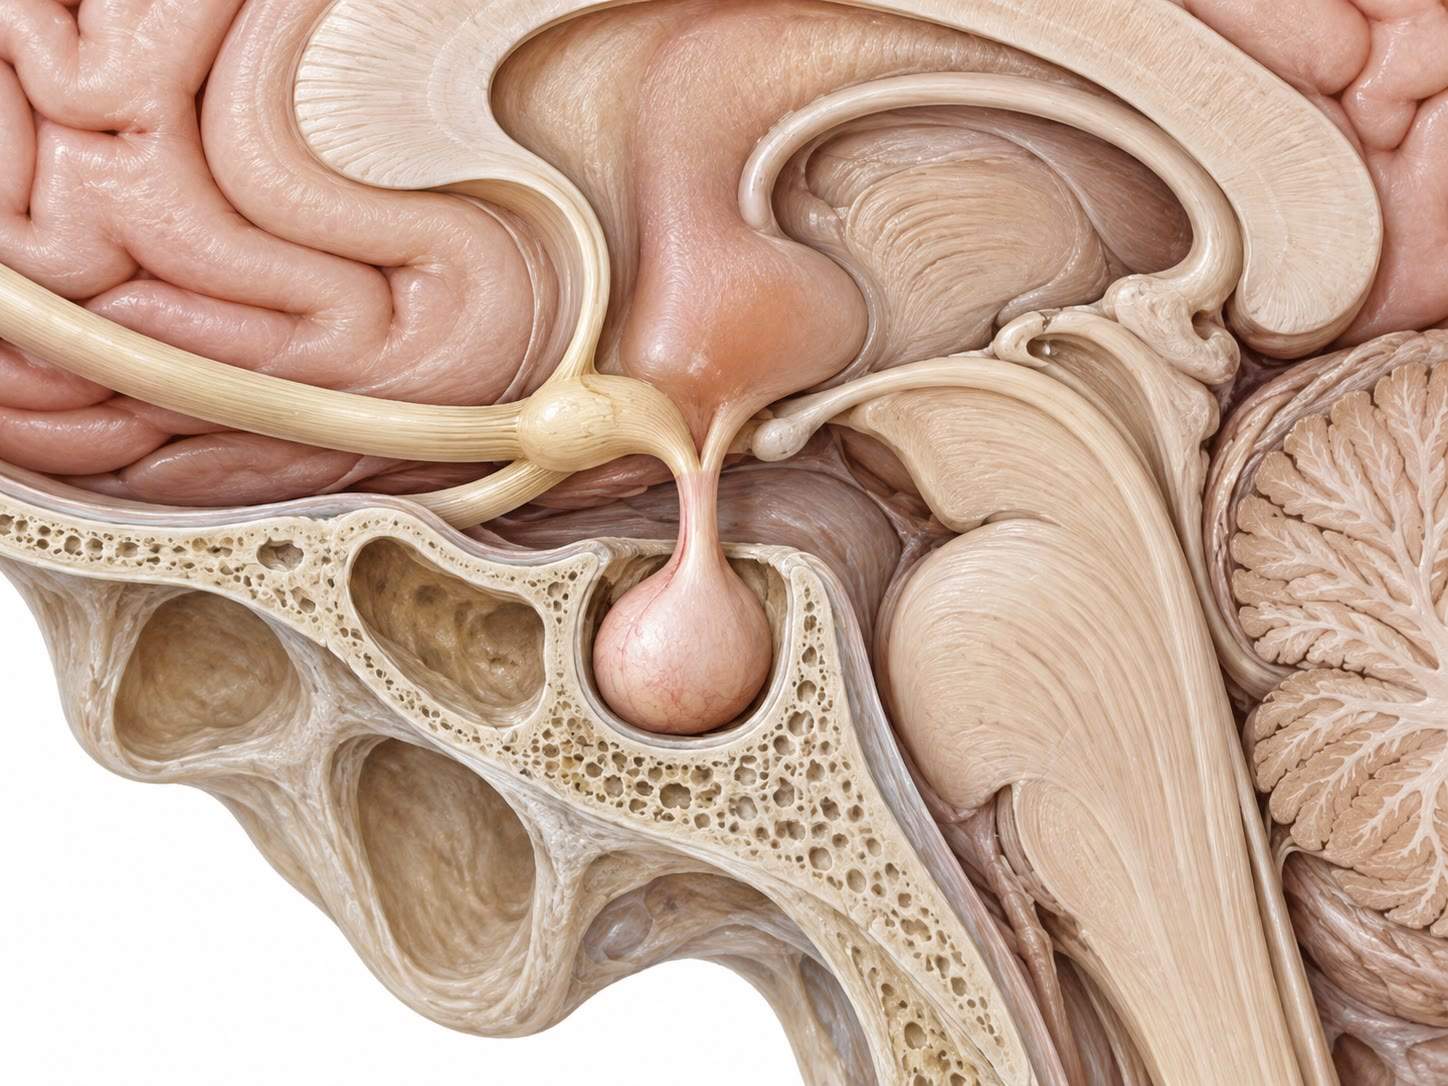
\includegraphics[width=0.55\linewidth]{images/book4/ai/b4-09-hypothalamus-pituitary.jpg}

{\small La base del encéfalo en sección sagital: el hipotálamo arriba, el
tallo y la hipófisis en su alojamiento óseo --- el soporte material del
eje.}
\end{omfigure}

\section{El varón: control tónico}

\begin{proposition}[El control del testículo]\label{prop:b2:reproductive-hormones:testis}
\index{testosterona}\index{inhibina}
La LH actúa sobre las \omterm{def:b2:mammal-reproduction:testis}{células de Leydig}, que fabrican
\emph{testosterona} (\qtyrange{3}{10}{ng/mL} en la sangre de un hombre
adulto, cien veces más dentro del \omterm{def:b2:mammal-reproduction:testis}{testículo}). La FSH actúa sobre las
\omterm{def:b2:mammal-reproduction:testis}{células de Sertoli}, que --- con la testosterona local --- sostienen la
\omterm{def:b2:mammal-reproduction:testis}{espermatogénesis} y secretan \emph{inhibina}. La testosterona ejerce una
retroalimentación sobre el hipotálamo y la hipófisis que mantiene baja la
LH; la inhibina, sobre la hipófisis, mantiene baja la FSH. Ambos bucles
son \emph{negativos} y el sistema es \emph{tónico}: los niveles
hormonales fluctúan con los pulsos y a lo largo del día (son máximos por
la mañana), pero no siguen un ciclo, y los espermatozoides se producen de
forma continua. La testosterona construye y mantiene además las glándulas
y conductos accesorios, la barba, la voz, el músculo y el hueso, la
producción de glóbulos rojos y la libido, y en el feto formó el cuerpo
masculino (\cref{ch:b2:mammal-reproduction}). La castración la suprime:
la LH y la FSH se multiplican por varias veces por falta de
retroalimentación, y los caracteres secundarios regresan; la testosterona
inyectada restablece los caracteres --- pero no la fertilidad, porque
también suprime la LH y, con ella, la testosterona intratesticular que
necesita la \omterm{def:b2:mammal-reproduction:testis}{espermatogénesis}. Por eso los esteroides anabolizantes
vuelven infértiles a los hombres.
\end{proposition}
\begin{proof}[Evidencia]
Berthold (1849) castró gallos: sus crestas se encogieron y dejaron de
cantar y de pelear. Un \omterm{def:b2:mammal-reproduction:testis}{testículo} injertado en el abdomen de un castrado,
donde desarrolló un nuevo riego sanguíneo pero ningún nervio, restableció
la cresta, el canto y la pelea: el \omterm{def:b2:mammal-reproduction:testis}{testículo} actuaba a través de la
sangre --- la primera demostración de una secreción interna, cincuenta
años antes de la palabra hormona. La testosterona se aisló y se sintetizó
en 1935.
\end{proof}

\section{La mujer: un ciclo con un interruptor}

\begin{definition}[Los ciclos ovárico y uterino]\label{def:b2:reproductive-hormones:cycle}
\index{ciclo menstrual}\index{fase folicular}\index{fase lútea}\index{pico de LH}\index{endometrio}
El ciclo se cuenta desde el primer día de la menstruación y dura unos 28
días. \emph{Fase folicular} (días 1--14): la FSH, liberada de la
retroalimentación por la muerte del \omterm{def:b2:mammal-reproduction:ovary}{cuerpo lúteo} anterior, recluta una
cohorte de \omterm{def:b2:mammal-reproduction:ovary}{folículos}; estos secretan \emph{estradiol}, que aumenta de
forma sostenida; el estradiol y la inhibina reducen la FSH, y solo el
\omterm{def:b2:mammal-reproduction:ovary}{folículo} con más receptores de FSH sobrevive a esa caída --- el \omterm{def:b2:mammal-reproduction:ovary}{folículo}
dominante. En el útero, el estradiol reconstruye el \emph{endometrio} (la
fase proliferativa) y fluidifica el moco cervical. \emph{\omterm{def:b2:mammal-reproduction:ovary}{Ovulación}}
(día 14): cuando el estradiol se ha mantenido por encima de unos
\qty{200}{pg/mL} durante un día y medio, su retroalimentación sobre el
hipotálamo y la hipófisis pasa de negativa a \emph{positiva}; la LH se
multiplica por diez en un día --- el \emph{pico de LH} --- y unas 36 horas
después de su inicio el \omterm{def:b2:mammal-reproduction:ovary}{folículo} se rompe y libera el ovocito. \emph{Fase
lútea} (días 15--28): el \omterm{def:b2:mammal-reproduction:ovary}{folículo} vacío se convierte en el \omterm{def:b2:mammal-reproduction:ovary}{cuerpo lúteo},
que bajo la LH secreta \emph{progesterona} (\qtyrange{10}{20}{ng/mL}) y
estradiol; la progesterona vuelve secretor el endometrio, espesa el moco,
eleva la temperatura corporal basal en \qty{0.3}{\celsius} y, con el
estradiol, suprime la LH y la FSH. El \omterm{def:b2:mammal-reproduction:ovary}{cuerpo lúteo} vive unos 14 días;
salvo que la hCG de un embrión lo rescate, regresa, la progesterona y el
estradiol caen, el endometrio se desprende (\emph{menstruación}), la FSH
aumenta y comienza el ciclo siguiente. La fase lútea dura fijamente 14
días; la variación de la duración del ciclo es variación de la fase
folicular.
\end{definition}

\begin{omfigure}
\begin{tikzpicture}
\begin{axis}[
  width=0.94\linewidth, height=6.4cm,
  axis x line=bottom, axis y line=left,
  xmin=0, xmax=28, ymin=0, ymax=1.15,
  xlabel={día del ciclo}, ylabel={hormonas (relativas al máximo)},
  xlabel style={font=\small, at={(axis description cs:0.5,-0.11)}, anchor=north},
  ylabel style={font=\small},
  tick label style={font=\small}, xtick={0,7,14,21,28}, ytick={0,0.5,1},
  legend style={font=\scriptsize, at={(0.5,-0.25)}, anchor=north, draw=none, legend columns=4},
  clip=false,
]
\addplot[very thick, omThm, domain=0:28, samples=120] {0.1 + 0.9*exp(-((x-14)^2)/0.9)};
\addlegendentry{LH}
\addplot[very thick, omProp, domain=0:28, samples=120] {0.35*exp(-x/6) + 0.15 + 0.35*exp(-((x-14)^2)/1.2)};
\addlegendentry{FSH}
\addplot[very thick, omDef, domain=0:28, samples=160] {0.1 + 0.9*exp(-((x-12.5)^2)/6) + 0.4*exp(-((x-21)^2)/12)};
\addlegendentry{estradiol}
\addplot[very thick, omExo!70!black, domain=0:28, samples=160] {0.03 + 0.97*exp(-((x-21)^2)/12)*(x>14)};
\addlegendentry{progesterona}
\draw[dashed, gray] (axis cs:14.5,0) -- (axis cs:14.5,1.1); \node[font=\scriptsize, anchor=south] at (axis cs:14.5,1.1) {ovulación};
\node[font=\scriptsize, anchor=north] at (axis cs:7,1.1) {fase folicular};
\node[font=\scriptsize, anchor=north] at (axis cs:21.5,1.1) {fase lútea};
\end{axis}
\end{tikzpicture}

{\small Las hormonas del ciclo. El estradiol del \omterm{def:b2:mammal-reproduction:ovary}{folículo} en crecimiento
aumenta a lo largo de la \omterm{def:b2:reproductive-hormones:cycle}{fase folicular} y, superado un umbral, desencadena
el \omterm{def:b2:reproductive-hormones:cycle}{pico de LH}; la \omterm{def:b2:mammal-reproduction:ovary}{ovulación} se produce unas 36 horas después; el \omterm{def:b2:mammal-reproduction:ovary}{cuerpo
lúteo} secreta entonces progesterona durante dos semanas y muere.}
\end{omfigure}

\begin{omfigure}
\begin{tikzpicture}[every node/.style={font=\scriptsize}]
  % endometrium thickness over the cycle
  \draw[thick, ->] (0,0) -- (12.4,0) node[right] {día};
  \foreach \x/\l in {0/1, 2.1/5, 6.0/14, 12/28} \draw (\x,0.08) -- (\x,-0.08) node[below] {\l};
  \fill[omThm!25] (0,0) -- (0,1.4) .. controls (0.8,1.2) and (1.6,0.5) .. (2.1,0.35) -- (2.1,0) -- cycle;
  \fill[omDef!20] (2.1,0) -- (2.1,0.35) .. controls (3.5,0.6) and (5.2,1.3) .. (6.0,1.5) -- (6.0,0) -- cycle;
  \fill[omExo!35] (6.0,0) -- (6.0,1.5) .. controls (8,1.8) and (11,1.9) .. (12,1.6) -- (12,0) -- cycle;
  \node at (1.0,1.8) {menstruación};
  \node at (4.0,1.8) {proliferativa (estradiol)};
  \node at (9,2.2) {secretora (progesterona): glándulas, glucógeno, arterias espirales};
  \node[anchor=east] at (-0.1,0.8) {endometrio};
\end{tikzpicture}

{\small El ciclo uterino. El \omterm{def:b2:reproductive-hormones:cycle}{endometrio} se desprende en la menstruación, se
reconstruye bajo el estradiol y se vuelve secretor bajo la progesterona,
preparado para recibir un \omterm{def:b2:mammal-reproduction:implantation}{blastocisto} hacia el día 21; cuando la
progesterona cae, vuelve a desprenderse.}
\end{omfigure}

\begin{omfigure}
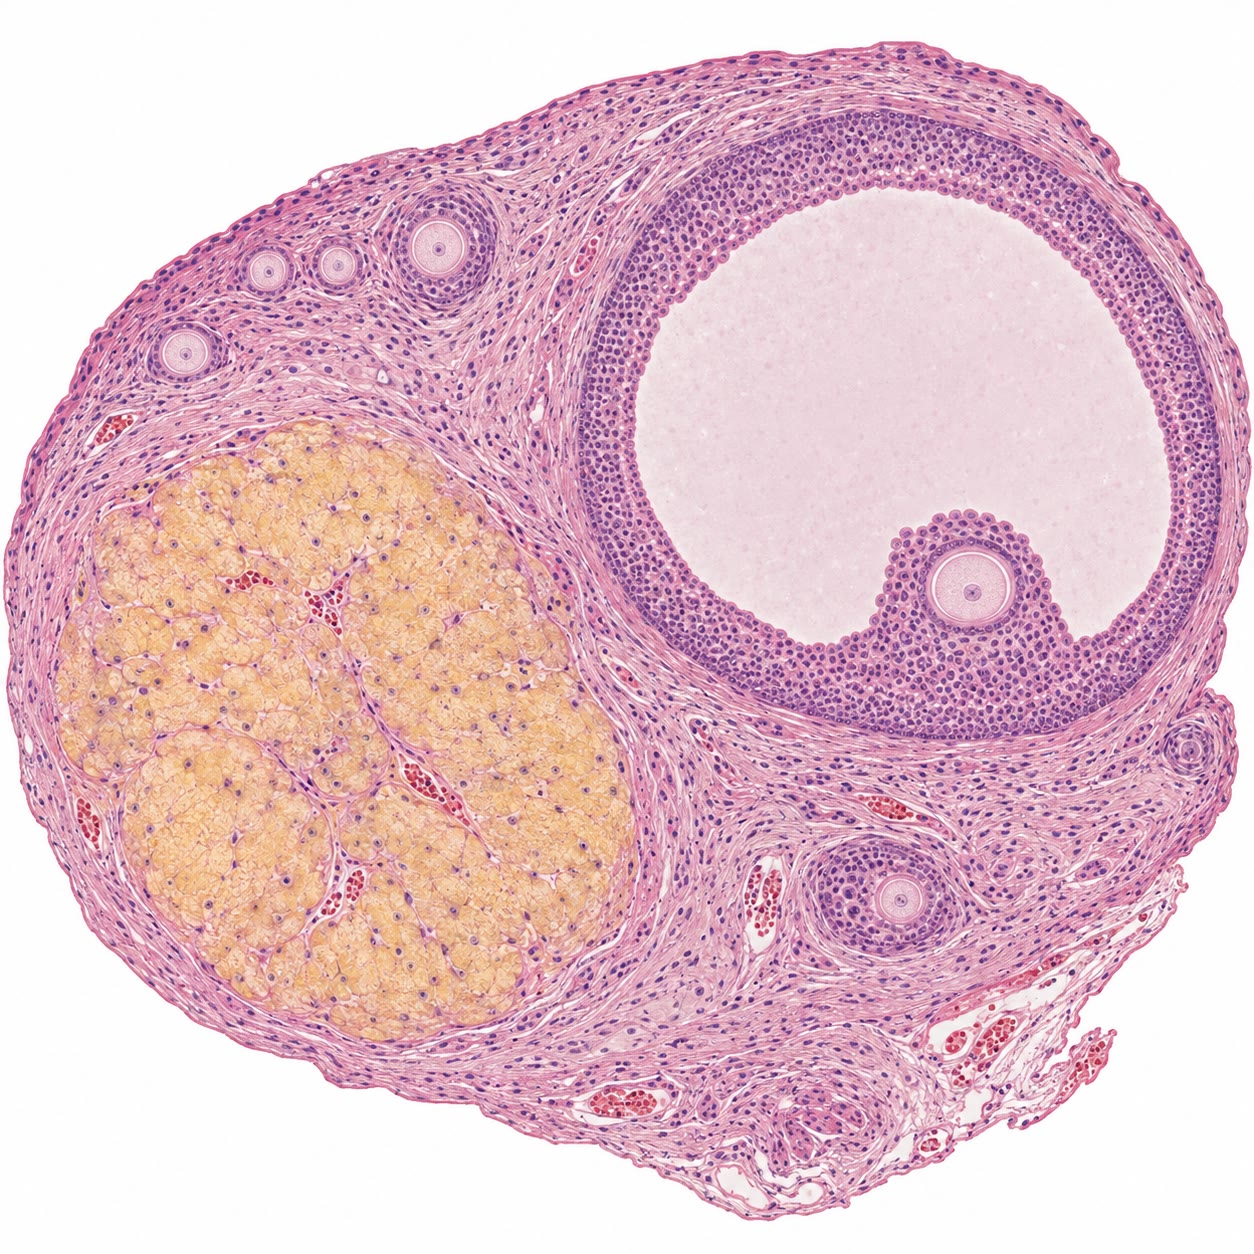
\includegraphics[width=0.46\linewidth]{images/book4/ai/b4-09-ovary-histology.jpg}

{\small Un ovario en sección: un \omterm{def:b2:mammal-reproduction:ovary}{folículo} maduro con su cavidad y su
ovocito, pequeños \omterm{def:b2:mammal-reproduction:ovary}{folículos} primordiales bajo la superficie y un \omterm{def:b2:mammal-reproduction:ovary}{cuerpo
lúteo} de un ciclo anterior.}
\end{omfigure}

\begin{theorem}[El paso de la retroalimentación negativa a la positiva]\label{thm:b2:reproductive-hormones:switch}
\index{retroalimentación positiva!pico de LH}
El estradiol, a los niveles bajos del comienzo de la \omterm{def:b2:reproductive-hormones:cycle}{fase folicular},
inhibe la LH y la FSH; el estradiol por encima de unos
\qty{200}{pg/mL}, mantenido durante más de unas \qty{36}{h}, hace lo
contrario: hace que el hipotálamo libere una descarga de GnRH y que la
hipófisis responda con una subida de la LH de diez veces. El mecanismo es
un cambio de signo, no de magnitud: una dosis alta y sostenida induce en
la hipófisis una gran reserva de LH y una sensibilidad aumentada a la
GnRH, y en el hipotálamo (a través de las neuronas de kisspeptina) el paso
del generador de pulsos de GnRH a un modo de descarga. El interruptor
convierte una señal graduada --- cuánto estradiol produce el \omterm{def:b2:mammal-reproduction:ovary}{folículo} ---
en un suceso de todo o nada ajustado al día, que es lo que requiere la
\omterm{def:b2:mammal-reproduction:ovary}{ovulación}; y como solo un \omterm{def:b2:mammal-reproduction:ovary}{folículo} grande y maduro puede sostener
\qty{200}{pg/mL}, el pico solo se dispara cuando hay un óvulo listo para
ser liberado. Una vez producida la \omterm{def:b2:mammal-reproduction:ovary}{ovulación}, la progesterona del \omterm{def:b2:mammal-reproduction:ovary}{cuerpo
lúteo} restablece la retroalimentación negativa y no sigue un segundo
pico.
\end{theorem}
\begin{proof}[Evidencia]
En mujeres y monas con el eje suprimido, una infusión de estradiol que
eleva el nivel plasmático por encima de \qty{200}{pg/mL} durante dos días
va seguida de un \omterm{def:b2:reproductive-hormones:cycle}{pico de LH}; la misma cantidad administrada durante un
día, o un nivel inferior durante tres, no. La progesterona administrada
antes de la infusión bloquea el pico; administrada a la vez, lo adelanta
y lo amplifica. El umbral de dosis y de duración reproduce el calendario
del pico natural a partir de la subida natural del estradiol.
\end{proof}

\section{La anulación del ciclo}

\begin{proposition}[Embarazo, lactancia, menopausia]\label{prop:b2:reproductive-hormones:overrides}
\index{gonadotropina coriónica humana}\index{menopausia}
Un embrión que se implanta secreta \emph{hCG}, una hormona análoga a la
LH que se une al receptor de la LH y mantiene vivo y secretor al \omterm{def:b2:mammal-reproduction:ovary}{cuerpo
lúteo} más allá de sus catorce días; hacia la semana diez la propia
\omterm{def:b2:mammal-reproduction:placenta}{placenta} produce progesterona y estrógenos suficientes para mantener el
embarazo, y el \omterm{def:b2:mammal-reproduction:ovary}{cuerpo lúteo} deja de ser indispensable. Durante todo el
embarazo, los esteroides elevados mantienen la LH y la FSH en cero: no
crece ningún \omterm{def:b2:mammal-reproduction:ovary}{folículo} ni se produce ninguna \omterm{def:b2:mammal-reproduction:ovary}{ovulación}. Tras el parto, la
succión eleva la prolactina y ralentiza los pulsos de GnRH, y la
\omterm{def:b2:mammal-reproduction:ovary}{ovulación} permanece suprimida durante meses. En la \emph{menopausia} la
reserva de \omterm{def:b2:mammal-reproduction:ovary}{folículos} se agota: el estradiol y la inhibina caen y, sin
nada que ejerza retroalimentación, la LH y la FSH suben hasta diez veces
su nivel anterior y se quedan ahí --- la firma de una glándula que ha
dejado de responder.
\end{proposition}

\begin{proposition}[Anticoncepción y reproducción asistida]\label{prop:b2:reproductive-hormones:clinic}
\index{anticoncepción!hormonal}\index{fecundación in vitro}
La píldora combinada aporta cada día un estrógeno sintético y un
progestágeno: el nivel constante de esteroides mantiene bajas la FSH y la
LH, no se recluta ningún \omterm{def:b2:mammal-reproduction:ovary}{folículo}, no se produce la subida del estradiol y
el pico nunca se dispara; el progestágeno espesa además el moco cervical.
La pausa de siete días permite que el \omterm{def:b2:reproductive-hormones:cycle}{endometrio} sangre; olvidar las
píldoras más de dos días seguidos deja escapar la FSH, y puede crecer un
\omterm{def:b2:mammal-reproduction:ovary}{folículo}. La anticoncepción de urgencia retrasa unos días el pico con una
dosis elevada de progestágeno. En la \emph{\omterm{prop:b2:reproductive-hormones:clinic}{fecundación in vitro}} el eje se
conduce en sentido contrario: la FSH diaria durante diez días anula la
selección de un único \omterm{def:b2:mammal-reproduction:ovary}{folículo} dominante y hace madurar diez o más; un
antagonista de la GnRH impide un pico espontáneo prematuro; una inyección
de hCG sustituye al pico, y los ovocitos se recogen entre 34 y 36 horas
después, justo antes de que se hubieran liberado; se fecundan en la placa
y se transfieren uno o dos embriones, y el resto se congela. En el hombre,
la testosterona exógena o un análogo de la GnRH suprimen la
\omterm{def:b2:mammal-reproduction:testis}{espermatogénesis} al suprimir la LH --- el principio de un anticonceptivo
hormonal masculino, todavía no comercializado. Todo esto es el eje de la
primera sección, leído al revés.
\end{proposition}

\section{Ejercicios}

\begin{exercise}[$\star$]\label{exo:b2:reproductive-hormones:1}
Dibújese el eje del varón: los tres niveles, las cuatro hormonas, los dos
bucles de retroalimentación y las células sobre las que actúa cada
hormona.
\end{exercise}

\begin{exercise}[$\star$]\label{exo:b2:reproductive-hormones:2}
Dense las fases de los ciclos ovárico y uterino con sus días y la hormona
que domina en cada una.
\end{exercise}

\begin{exercise}[$\star$]\label{exo:b2:reproductive-hormones:3}
Explíquese cómo impide la \omterm{def:b2:mammal-reproduction:ovary}{ovulación} la píldora combinada, y por qué se
produce un sangrado en la semana sin píldoras.
\end{exercise}

\begin{exercise}[$\star$]\label{exo:b2:reproductive-hormones:4}
¿Qué les ocurre a la LH, a la FSH y a los caracteres sexuales secundarios
de un varón adulto castrado? ¿Cuáles de estos efectos revierte la
testosterona inyectada, y cuáles no?
\end{exercise}

\begin{exercise}[$\star\star$]\label{exo:b2:reproductive-hormones:5}
Los pulsos de GnRH llegan cada \qty{90}{min} en la \omterm{def:b2:reproductive-hormones:cycle}{fase folicular} y cada
\qty{4}{h} en la \omterm{def:b2:reproductive-hormones:cycle}{fase lútea}. ¿Cuántos pulsos hay al día en cada una? La
hipófisis favorece la LH con pulsos rápidos y la FSH con pulsos lentos:
¿qué gonadotropina debería subir primero cuando muere el \omterm{def:b2:mammal-reproduction:ovary}{cuerpo lúteo}, y
por qué es esa la adecuada?
\end{exercise}

\begin{exercise}[$\star\star$]\label{exo:b2:reproductive-hormones:6}
Conviértanse \qty{200}{pg/mL} de estradiol (masa molar
\qty{272}{g/mol}) en \unit{pmol/L}, y \qty{15}{ng/mL} de
progesterona (\qty{314}{g/mol}) en \unit{nmol/L}. ¿Cuántas moléculas de
estradiol hay en un microlitro de plasma en el umbral del pico?
\end{exercise}

\begin{exercise}[$\star\star$]\label{exo:b2:reproductive-hormones:7}
Los ciclos de una mujer duran 35 días. Dado que la \omterm{def:b2:reproductive-hormones:cycle}{fase lútea} es fija,
¿qué día ovula, y qué días son fértiles si los espermatozoides sobreviven
tres días y el óvulo uno? ¿Por qué falla el método del calendario en los
ciclos irregulares?
\end{exercise}

\begin{exercise}[$\star\star$]\label{exo:b2:reproductive-hormones:8}
Un embrión se implanta el día 21 de un ciclo de 28 días y su hCG, que
parte de \qty{1}{IU/L}, se duplica cada dos días. El \omterm{def:b2:mammal-reproduction:ovary}{cuerpo lúteo} necesita
unas pocas IU/L de hCG hacia el día 26 para sobrevivir. ¿Llega a tiempo
el embrión? ¿Qué ocurriría si la \omterm{def:b2:mammal-reproduction:implantation}{implantación} se retrasara al día 25?
\end{exercise}

\begin{exercise}[$\star\star$]\label{exo:b2:reproductive-hormones:9}
Enúnciese qué mostró el experimento de Knobil y qué descartó, y
predígase el efecto de administrar a una mujer un agonista de la GnRH de
acción prolongada durante un mes: sobre la LH, sobre el estradiol y
sobre el \omterm{def:b2:reproductive-hormones:cycle}{endometrio}.
\end{exercise}

\begin{exercise}[$\star\star\star$]\label{exo:b2:reproductive-hormones:10}
En el modelo de receptores, tómense $s = 100$ receptores por hora, $d =
\qty{0.5}{h^{-1}}$ e $iH = \qty{6}{h^{-1}}$ mientras la hormona está
presente. Calcúlese el número de receptores en estado estacionario sin
hormona y con hormona continua. Con un pulso de dos minutos cada hora,
calcúlense el número de receptores perdidos por pulso y la fracción del
déficit recuperada antes del pulso siguiente, y dedúzcase el nivel en
torno al cual se estabiliza la reserva.
\end{exercise}

\begin{exercise}[$\star\star\star$]\label{exo:b2:reproductive-hormones:11}
Una mujer posmenopáusica tiene la LH y la FSH diez veces por encima del
nivel de una mujer joven y un estradiol muy bajo; una mujer con un tumor
hipofisario secretor de prolactina tiene la LH baja, el estradiol bajo y
no tiene ciclos; una mujer con un tumor de células de la granulosa tiene
el estradiol alto, la LH baja y no tiene ciclos. Explíquese cada perfil a
partir del eje.
\end{exercise}

\begin{exercise}[$\star\star\star$]\label{exo:b2:reproductive-hormones:12}
``La misma hormona inhibe y después desencadena el \omterm{def:b2:reproductive-hormones:cycle}{pico de LH}.''
Explíquese cómo puede tener el estradiol ambos efectos, por qué la
\omterm{def:b2:mammal-reproduction:ovary}{ovulación} necesita un interruptor y no un regulador gradual, y qué
fallaría con un regulador gradual.
\end{exercise}

\section{Problema: un ciclo medido}

\begin{problem}[{Problema de fin de semana --- se leen las mediciones
hormonales diarias de un ciclo para hallar sus fases, el día de la
ovulación y la ventana fértil; se calculan el umbral del pico, el reloj
del cuerpo lúteo y el rescate por la hCG; el modelo de receptores explica
a Knobil; y el eje se conduce al revés en la clínica, hasta llegar al día
de la ovulación, la duración de la fase lútea, la ventana fértil y el
umbral del pico}]
\label{pb:b2:reproductive-hormones:1}
Se tomaron muestras de sangre en días seleccionados del ciclo de una
mujer:

\begin{center}
\small
\begin{tabular}{lcccccccccc}
\hline
día & 1 & 5 & 8 & 11 & 12 & 13 & 14 & 15 & 21 & 27 \\
\hline
estradiol (\unit{pg/mL}) & 40 & 60 & 110 & 210 & 260 & 310 & 220 & 150 & 160 & 50 \\
LH (\unit{IU/L}) & 5 & 5 & 6 & 7 & 8 & 20 & 65 & 15 & 4 & 4 \\
progesterona (\unit{ng/mL}) & 0.5 & 0.5 & 0.6 & 0.7 & 0.8 & 1.0 & 1.5 & 3 & 16 & 2 \\
temperatura (\unit{\celsius}) & 36.4 & 36.4 & 36.4 & 36.4 & 36.4 & 36.4 & 36.4 & 36.5 & 36.8 & 36.7 \\
\hline
\end{tabular}
\end{center}

La menstruación empezó el día 1 y de nuevo el día 29.

\medskip
\noindent\textbf{Parte I --- Leer el ciclo.}
\begin{enumerate}
  \item Identifíquense en la tabla las \omterm{def:b2:reproductive-hormones:cycle}{fases folicular} y lútea, con la
        hormona que marca cada una.
  \item ¿Qué día alcanzó su máximo el \omterm{def:b2:reproductive-hormones:cycle}{pico de LH}? ¿Cuándo se produjo la
        \omterm{def:b2:mammal-reproduction:ovary}{ovulación}?
  \item ¿Cuánto duró la \omterm{def:b2:reproductive-hormones:cycle}{fase lútea}? ¿Es coherente con la vida del \omterm{def:b2:mammal-reproduction:ovary}{cuerpo
        lúteo}?
  \item Explíquese el cambio de temperatura y por qué confirma la
        \omterm{def:b2:mammal-reproduction:ovary}{ovulación} pero no puede predecirla.
  \item ¿Qué días estuvo el estradiol por encima de \qty{200}{pg/mL}?
        Relaciónese esa duración con el pico.
  \item Dese la ventana fértil de este ciclo (espermatozoides, tres días;
        óvulo, un día).
\end{enumerate}

\medskip
\noindent\textbf{Parte II --- Cifras.}
\begin{enumerate}[resume]
  \item Conviértanse el estradiol del día 13 en \unit{pmol/L} y la
        progesterona del día 21 en \unit{nmol/L}.
  \item ¿Por qué factor aumentó la LH del día 12 al día 14? ¿Por qué cae
        tan deprisa después (la semivida de la LH es de alrededor de
        \qty{1}{h})?
  \item Si el ciclo siguiente de esta mujer tuviera una \omterm{def:b2:reproductive-hormones:cycle}{fase folicular} de
        21 días, ¿qué día ovularía y cuánto duraría el ciclo?
  \item Un embrión se implanta 7 días después de la \omterm{def:b2:mammal-reproduction:ovary}{ovulación}. ¿Qué día de
        este ciclo aparecería la hCG y, duplicándose cada dos días desde
        \qty{1}{IU/L}, qué nivel alcanzaría hacia el día 27?
  \item Explíquese por qué la progesterona de \qty{2}{ng/mL} del día 27
        muestra que no se implantó ningún embrión.
  \item ¿Cuáles habrían sido los valores de progesterona y de estradiol
        del día 27 si se hubiera implantado?
\end{enumerate}

\medskip
\noindent\textbf{Parte III --- Retroalimentación y pulsos.}
\begin{enumerate}[resume]
  \item Explíquese, con los signos de la retroalimentación, por qué la FSH
        es máxima al comienzo del ciclo y por qué normalmente solo
        sobrevive un \omterm{def:b2:mammal-reproduction:ovary}{folículo}.
  \item En el modelo de receptores con $s = 100$ por hora, $d =
        \qty{0.5}{h^{-1}}$ e $iH = \qty{6}{h^{-1}}$, calcúlese $R^*$ sin
        hormona y con hormona continua.
  \item Un pulso dura \qty{2}{min}. Partiendo del $R^*$ sin estimulación,
        ¿cuántos receptores retira un pulso (úsese la aproximación lineal
        $iHR\,\Delta t$)? ¿Qué fracción del déficit se recupera en la hora
        anterior al pulso siguiente (constante de tiempo $1/d$), y en torno
        a qué nivel se estabiliza la reserva?
  \item Úsense estas cifras para explicar el resultado de Knobil.
  \item A un hombre se le administra de forma continua un agonista de la
        GnRH por un cáncer de próstata. Predíganse su LH y su testosterona
        al cabo de un día y al cabo de un mes, y explíquese la
        diferencia.
  \item Las células de la granulosa de una mujer no fabrican inhibina.
        Predíganse su FSH y su LH, y la consecuencia para el reclutamiento
        de \omterm{def:b2:mammal-reproduction:ovary}{folículos}.
\end{enumerate}

\medskip
\noindent\textbf{Parte IV --- La clínica.}
\begin{enumerate}[resume]
  \item Para una \omterm{prop:b2:reproductive-hormones:clinic}{fecundación in vitro}, esta mujer recibe FSH a diario
        desde el día 2. Explíquese por qué maduran diez \omterm{def:b2:mammal-reproduction:ovary}{folículos} en lugar
        de uno.
  \item ¿Por qué se añade un antagonista de la GnRH desde el día 6, y qué
        ocurriría sin él?
  \item Se inyecta hCG cuando los \omterm{def:b2:mammal-reproduction:ovary}{folículos} están maduros; los ovocitos se
        recogen 35 horas después. Justifíquese ese plazo con la tabla.
  \item Se recogen diez ovocitos; el \qty{70}{\%} se fecunda, el
        \qty{40}{\%} de los embriones llega al estadio de \omterm{def:b2:mammal-reproduction:implantation}{blastocisto} y
        cada \omterm{def:b2:mammal-reproduction:implantation}{blastocisto} transferido se implanta con probabilidad $0.35$.
        ¿Número esperado de \omterm{def:b2:mammal-reproduction:implantation}{blastocistos}? ¿Probabilidad de al menos un
        embarazo si se transfieren dos?
  \item Explíquese por qué la píldora combinada, tomada por esta mujer,
        habría dado una tabla sin \omterm{def:b2:reproductive-hormones:cycle}{pico de LH} y sin subida de la
        progesterona.
  \item Un anticonceptivo masculino basado en un antagonista de la GnRH
        suprimiría también la testosterona. ¿Qué debe administrarse con
        él, y por qué administrarlo no restablece la producción de
        espermatozoides?
  \item Enúnciese el resultado: el día de la \omterm{def:b2:mammal-reproduction:ovary}{ovulación}, la duración de la
        \omterm{def:b2:reproductive-hormones:cycle}{fase lútea}, la ventana fértil, y el umbral y la duración del
        estradiol que desencadenaron el pico.
\end{enumerate}
\end{problem}
